% Appendices are set up same as chapter sections
\chapter{Appendix - Deep analysis of users problems and needfinding}

\section{User Benchmarking and Need-Finding}
The first deliverable of the fall quarter concerning our corporate project was the benchmarking and need-finding deliverable.  Current systems and technology were to be researched to see what is available to complete the benchmarking task.  User interviews and user personas were to be conducted and developed, respectively, to inform our team and audience on what needs our solution needs to be addressing. 

\section{Need-Finding}
The solution to a problem needs to address the gaps that exist within the current systems. In order to find these gaps, our team had to extensive need finding by conducting user interviews with different potential users as well as experts in the field.  Each interview gave us some more detail into who our user would be and how to go about developing our personas.

\subsection{Expert Interviews}
To begin the need-finding process, we wanted to investigate what research projects had been pursued within the aerospace industry. Two experts, one from Boeing and the other from Oregon State University shared their work experience and its motivation with us. 

\subsubsection{Dianne McMullin, Human Factors Engineer at Boeing}
\begin{figure}[h]
  \centering
     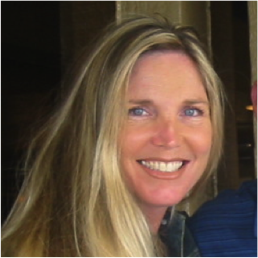
\includegraphics[width=7cm]{images/image020}
  \label{fig:20}
\end{figure}

Dianne McMullin is a technical fellow in Human Factors Engineer at Boeing and worked on the 787 Assistive Technology Design.  She has been working on this problem for over 15 years.  Since she is currently working on a project with Embraer to better the flying experience for the aging passenger, she had a lot of fresh knowledge that proved to be very relevant to our work. She shared with us some of the major restrictions we need to be conscious of such when designing something for the airline industry. These include:	
\begin{list}{-}{}
  \item Maintain the number of seats. Airlines, and consequently airplane manufacturers, want the maximum number of seats possible to maximize profit.
  \item While in the air, space is more expensive than most expensive real estate in Tokyo, minimizing size is paramount.
  \item Weight is a critical factor, a solution cannot significantly add weight to the aircraft.
\end{list}

She was also able to share with us some touching points that she had encountered in her research and work.  These two aspects made the team think about our users in a new light and helped us empathize with the situation and feel the pain.  

\begin{list}{-}{}
  \item The utter sense of despair and helplessness when cane/crutches is taken away.
  \item Not traveling can mean not seeing kids or grandkids, missing weddings and vacations. It literally means giving up a piece of their life. Making this a better experience can, in essence, give back a little piece of that.
\end{list}

\subsection{Kate Hunter-Zaworksi, Director of National Center for Accessible Transportation}
\begin{figure}[h]
  \centering
     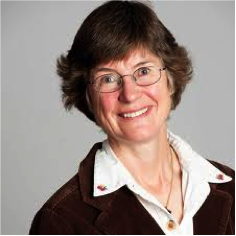
\includegraphics[width=7cm]{images/image021}
  \label{fig:21}
\end{figure}
Kate Hunter-Zaworski is the Director of the National Center for Accessible Transportation and also worked with Boeing on the 787 Assistive Technology Design.  She was able to give us some more places to contact, interesting facts that could be used to implement a design solution, and areas to start brainstorming.  Below is some of the food for thought she left us with:

\begin{list}{-}{}
  \item When considering the possibility of tying down wheelchairs within the cabin, the wheelchair’s impact capabilities are of prime concern. However, some wheelchairs are able to stand up to 20Gs while airplane seats can only support 16Gs.
  \item Folding canes and other mobility aids that can be stored within the cabin and remain accessible are interesting solutions to consider. 
  \item Why can’t you maneuver a wheelchair with only one hand?
\end{list}

\subsection{User Interviews}
User interviews were used to really get a sense for what the user experience was, allowing us to no longer rely on our own assumptions. Given that the problem statement does not state a type of disability to focus on, we strived to encompass as many different types of disabilities as possible, looking for overlaps within the experiences. The interviews not only gave us insight into where the pain point lie but also humanized the problem even more for us. Being able to talk to these users who both have to deal with these issues on a daily basis but are also invested in helping others navigate the traveling process was extremely rewarding. Their passion for the subject refueled our own. 

\subsection*{Wheelchair Users}
The motivation behind these interviews was to find areas where corrective actions can be implemented during the travel experience for a person in a wheelchair.

\subsubsection{Teri Adams, Assistant Director of Stanford Office of Accessible Education}
\begin{figure}[h]
  \centering
     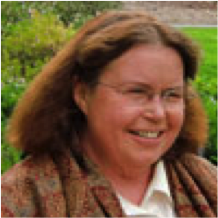
\includegraphics[width=7cm]{images/image022}
  \label{fig:22}
\end{figure}

Teri Adams is the Assistant Director of the Stanford Office of Accessible Education.  She is an avid traveler and utilizes a power wheelchair every day and a manual wheelchair on trips. She used to travel with her power wheelchair but stopped after having several instances where her chair came back from the cargo hold broken. The following are the main areas she highlighted within her interview:

\begin{figure}[h]
  \centering
     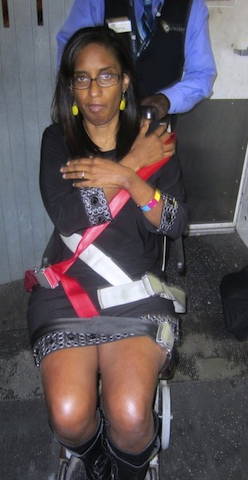
\includegraphics[width=7cm]{images/image023}
   \caption{Nicole Lemelle has Multiple Sclerosis and needs ad aisle chair to board the plane. Source: http://www.mynewnormals.com/aisle-chair/}
  \label{fig:23}
\end{figure}

\begin{list}{-}{}
  \item Highlighted the persistent problem of wheelchairs being broken, both in her experience as well as her friends'.
  \item Described the aisle chair used to move wheelchair users from their wheelchair into the airplane seat if they cannot do it themselves. It is an incredibly degrading and embarrassing process, as shown in Figure 3 4 because the chair is not designed to fit an average sized person. Usually the process takes place before boarding begins.
  \item Addressed the important issue of customer service's impact. The most dramatic horror stories she had came from a lack of training or knowledge from the flight crew.
  \item Enlightened us on the reality of seat preferences. We assumed that people with disabilities would always choose to sit by the aisle due to the ease of access but actually found that many prefer to sit in the window seat so that they do not have to get up and down every time someone from their row needs to walk around the cabin. This is something that was completely new to us.
  \item Emphasized the difficulty of reaching the controls while in flight and the need for a more accessible and intuitive placement for them. 
\end{list}

\subsubsection{Scott Rains, Travel and Cruise Specialist for Disabled Persons}
\begin{figure}[h]
  \centering
     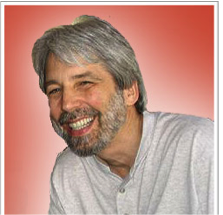
\includegraphics[width=7cm]{images/image024}
  \label{fig:24}
\end{figure}

Scott Rains is a paraplegic who is very passionate about the subject of disables traveling. He is a travel and cruise specialist and an avid travel blogger, providing a community of people with disabilities with tips on how to best navigate using the current solutions out there.  He travels multiple times a year for work and pleasure.  Scott was kind enough to connect us with multiple contacts that we were able to reach out to due to his wealth of knowledge on the subject matter.  The following were the main points that he stressed needed to be included in our design solution: 

\begin{list}{-}{}
  \item Surprisingly, hinged armrests are not the standard. There are many aircraft where they are not present, making the transfer of a disabled passenger infinitely more difficult. He recounted a friend’s experience of getting bumped into the armrest and needing to spend 2 weeks in the hospital as a result of the sore caused by the bump. 
  \item Even if hinged armrests are present, the hinges are often hard to find and the flight attendants are not familiar with how to operate them. It follows with other accessibility features such as additional seat belt extensions for lumbar support.
  \item All disabilities are different and thus they need different things. Wheelchair users often have customized cushions or seat pads that allow for more comfort. This type of solution should also be implemented in long duration flights. If people bring their own neck pillow, why not their own butt cushion?
  \item Reemphasized disabled passengers’ wishes to sit in the window seat also for the support the wall provides as well as not wanting to be disturbed when others need to walk around the cabin. Lack of accessible controls was also mentioned. 
\end{list}

\subsubsection{Jose Luis Naranjo, T6 Paraplegic}
\begin{figure}[h]
  \centering
     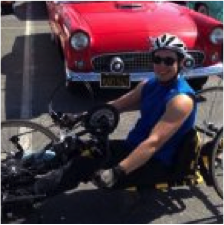
\includegraphics[width=7cm]{images/image025}
  \label{fig:25}
\end{figure}

Jose Luis Naranjo is a 28-year-old T6 paraplegic.  He studied engineering at MIT and now works in the bay area as a mechanical/aerospace engineer.  He gave us his view of the situation and applied his engineering knowledge to help us brainstorm other solutions.  His focus points were the following:

\begin{list}{-}{}
  \item Wheelchair storage in the cargo hold is extremely poor, they literally just throw the wheelchairs in there which allows them to shift around during flight. Very often chairs are broken. 
  \item Flight crew also does not know how to operate the wheelchairs and have tried to fold a non-foldable wheelchair before, resulting in damaged wheelchairs.
  \item He uses the aisle chair very often and has noticed that because the center of gravity is very high on the aisle chair, it’s very easy to flip over and there is little sense of control.
  \item Sometimes only one side of the airplane has folding armrests. 
  \item Boarding processes are extremely rushed, the flight crew’s main priority is to get the plane out on time which has a huge impact on how much time they spend with the disabled passengers that need assistance. 
  \item Keeping track of belongings is extremely difficult, you must rely on a flight attendant to carry your luggage and then remove all loose items from the wheelchair prior to storing it. This lack of independence and control over one’s belongings is nerve-wracking.
  \item He is a frequently traveler and thus is aware of the preparations he must ensure before each flight, especially assuring that he does not have to use the restroom at any point. 
  \item A solution must allow for people to do as much as they can themselves, returning that lost sense of independence and control. “What little mobility I have left, I want to use.”
  \item A solution must ensure that disabled passengers are not being segregated from the rest of the population. They already know they’re different, they don’t need to be reminded. Inclusivity is key. 
\end{list}

\subsubsection{Cid Torquato, Municipal Department of People with Disabilities and Reduced Mobility}
\begin{figure}[h]
  \centering
     
\includegraphics[width=7cm]{images/image026}
  \label{fig:26}
\end{figure}

Cid Torquato is the Coordinator at the Municipal Department of People with Disabilities and Reduced Mobility in Sao Paulo, Brazil. He is paraplegic, and constantly travels to several countries due to his responsibilities in the department. The main points of the interview are as follows:

\begin{list}{-}{}
  \item There are many difficulties applying the law, people simply do not want to follow it.
  \item There is a lack of proper training (and even good will) for many people involved in the flight experience.
  \item There are some alternatives to the use of bathrooms for people with reduced mobility, including drastic ones like using a catheter to collect urine, diapers or even plugs. Due to the discomfort of using these solutions, people still prefer to use the airplane bathroom.
  \item Usually, security will just use the hand metal detector and will not ask for the disabled to get up off the wheelchair. However, the interviewee had an awful experience during one of his travels where they forced him to do so, even though he cannot move. He had to make his companion make a space between his back and the chair to show to security there was in fact, nothing to hide.
  \item Some airlines use contractors to handle people with disabilities, where trained people help with transportation and other needs of the passenger.
  \item There is a lack of precise information about what can or cannot be done while boarding a reduced mobility passenger. Sometimes the airline does not allow the passenger to take his/her own wheelchair through the jet way to they airplane, stating that only the airport wheelchair is allowed even though the common procedure is to pull up at the front door of the airplane and change into the aisle chair. 
\end{list}

\subsubsection{Nanci Linke-Ellis, Board of Trustees for HLAA}

\begin{figure}[h]
  \centering
     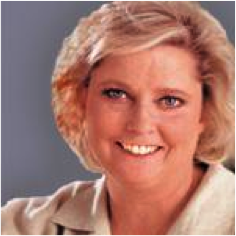
\includegraphics[width=7cm]{images/image027}
  \label{fig:27}
\end{figure}

Nanci Linke-Ellis is on the Board of Trustee for Hearing Loss Association of America and is a deaf traveler. She was able to give us more information about where corrective actions could be applied in the travel experience specifically concerning the deaf passenger. These are some of the problems she brought to our attention more than before:

\begin{list}{-}{}
  \item The customer service element is absolutely huge and causes a great deal of problems. Once, she approached the gate agent to inform her that she was deaf and would need to be notified of any announcements. The gate agent then asked her if she needed a wheelchair. Flight attendants do not know how to react or are uneducated about dealing with persons with disabilities. 
  \item As a disabled traveler, it is important to make the flight crew aware of the problem but also present a possible solution. 
  \item Planes, airports, terminals, etc. need more signage and to be more visual with instructions. This not only affects the deaf but also all passengers struggling to hear information over the loud background noise found in airports. Using a smartphone app could be an interesting solution
  \item Increasing independence is key. 
\end{list}

\subsection*{Blind User}
\subsubsection{Cheryl Echevarria, President of NFB Travel and Tourism Division}
\begin{figure}[h]
  \centering
     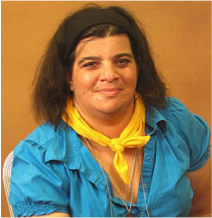
\includegraphics[width=7cm]{images/image028}
  \label{fig:28}
\end{figure}

Cheryl Echevarria is the President of NFB Travel and Tourism Division and owns her own travel agency that specializes in assisting blind travelers.  She shared with us the independence that blind persons have while travelling due to advancements in education for the blind and support for the blind as well as assistive technologies that are available.  She highlighted some of the main points that were already suggested by our previous interviews adding the following:

\begin{list}{-}{}
  \item Customer service is a major factor that can make or break an experience. The disabled person must be aware of the rules and be willing to teach uneducated flight crew about what is allowed during flight (such as leaving your cane under your seat). Blind people would most likely not be a target user given the range of technologies already available.
\end{list}

\subsection{Flight Crew}

\begin{figure}[h]
  \centering
     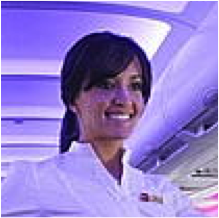
\includegraphics[width=7cm]{images/image029}
   \caption{Nikole Rubyn Virgin America Founding Flight Attendant}
  \label{fig:29}
\end{figure}

\begin{figure}[h]
  \centering
     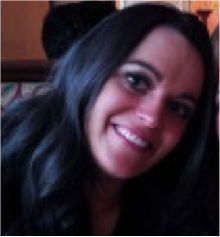
\includegraphics[width=7cm]{images/image030}
   \caption{Dena Silva-Heath Alaska Airlines Flight Attendant}
  \label{fig:30}
\end{figure}

\begin{figure}[h]
  \centering
     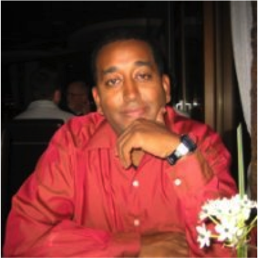
\includegraphics[width=7cm]{images/image031}
   \caption{Yonatan Godefa Virgin America Gate Agent}
  \label{fig:31}
\end{figure}

Interviewing potential users made us realize there were also other major stakeholders that had to be considered when designing a solution: the cabin crew. Not only does the cabin crew have to interact with disabled passengers on an every day basis but their actions are often fueled by motivations that can contradict providing the best assistance possible to the disabled passengers. We spoke with two flight attendants and a gate agent to get a better sense of what their pain points were, what they perceived the pain points to be for the disabled passenger and their motivations when executing tasks on the job. These findings can be broken down into two different areas of concern, the airports and the airplane. 

\subsubsection{Airport}
\begin{list}{-}{}
  \item Not all the airports are ready to receive disabled passengers; some do not have the appropriate equipment or personnel.
  \item Some airports do not have enough equipment for disabled. Once, one of the flight attendants waited 40 minutes for the lift, “airport elevator on the runway”, to disembark the disabled.
  \item The aisle chair is too small for most passengers.
\end{list}

\subsubsection{Airplane}
\begin{list}{-}{}
  \item Not all the armrest are retractable, in some aircraft just the ones on the first and the second rows are.
  \item The lavatory is too small for the aisle chair, so often the disabled have to use it with the door open.
  \item For blind people they can provide the safety procedures in Braille. Little known fact, however, is that not many blind people actually know Braille.
  \item For deaf people there isn’t any special equipment, the crew members have to speak really close so the disabled can read their lips. 
  \item People with no chest mobility can use a special belt, but sometimes the family doesn’t want it or the flight crew isn’t aware of its existence.
  \item Paralympics athletes can usually get to their seat on their own and thus they can allow more disabled passengers on the plane when they’re flying. Usually the number allowed is one third of the number of crewmembers.
\end{list}

\subsubsection{Miscellaneous}
\begin{list}{-}{}
  \item The disabled feels humiliated for being carried thought the aisle.
  \item A recently disabled person is usually more dependent and more uncomfortable with the situation.
  \item Many people do not prepare sufficiently for the flight. They either do not have credit cards to purchase food onboard or don’t realize they should go to the bathroom beforehand. The gate agents can play a role in aiding passengers prepare. 
  \item The flight crew has another 140 passengers they must cater to throughout the flight, making it impossible for them to dedicate a significant amount of time to assisting disabled passengers.
\end{list}

\subsection{Observations}
In order to get a complete picture of what the traveling experience entails in general as well as how it differs for disabled passengers, our team decided to use their travels as an opportunity to delve deeper into the topic. Six different people from USP made many of the following observations on October 2013. Both the teaching team and the students travelled from Palo Alto to São Paulo (GRU) via San Francisco (SFO) or San Jose (SJO) with connections in Dallas (DFW). Most of them were on different flights and got to experience different situations. Included are also observations conducted by the Stanford team during their flight home for Thanksgiving.

\subsubsection{Outside the Airport}
\begin{list}{-}{}
  \item It is difficult to find a cab in smaller cities (an accessible taxi would be even more difficult).
  \item Walking within the city of Palo Alto was not a good experience, especially because sidewalks suddenly disappeared without any indication whatsoever. Urban planners really must take people with disabilities into account when designing urban layouts.
  \item Ticket vending machines at Caltrain/BART are not suited for people with disabilities, it would be extremely hard for someone in a wheelchair to reach and purchase a ticket.
  \item Lack of signage makes it very difficult to travel by train, especially if one has any hearing loss (or doesn’t speak English fluently).
  \item The train and bus used to get to the San Jose airport do not offer adequate space for storing luggage near the seats reserved for people with disabilities.
  \item Getting in and out of the train is difficult because of the stairs and also because of the short time to embark.
  \item There are no people assisting passengers to embark the train/bus.
  \item There are not sufficient handles to hold on to on the train. This is a huge issue if one does not have perfect balance. 
\end{list}

\subsubsection{Inside the Airport}
\begin{list}{-}{}
  \item There are some boarding assisting areas inside the airport and dedicated waiting lines for people with reduced mobility, as seen in Figure 3 5.

\begin{figure}[h]
  \centering
     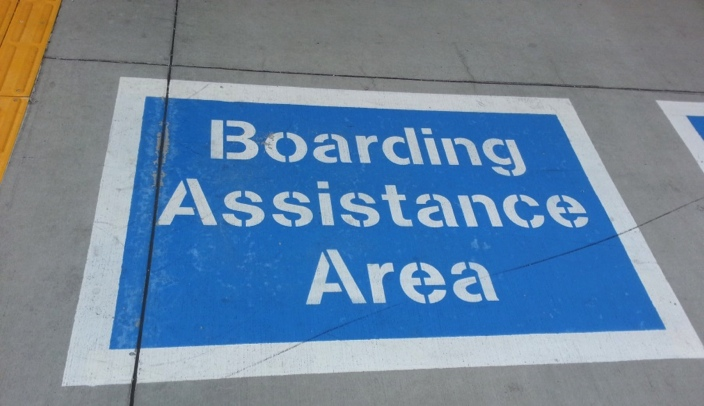
\includegraphics[width=7cm]{images/image032}
   \caption{From L to R: Boarding assistance area and dedicated waiting line}
  \label{fig:32}
\end{figure}
\begin{figure}[h]
  \centering
     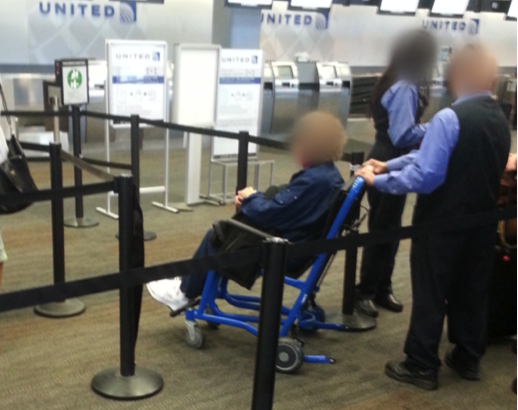
\includegraphics[width=7cm]{images/image033}
  \label{fig:33}
\end{figure}

  \item Finding the airline counter is not trivial, especially if one has a poor vision or is not familiar with the airport layout. There is not enough information displayed to make it an easy task.
  \item Check-in counters are not adapted for people with special needs. 
  \item Conventional check-in counter is too high for a person in a wheelchair. The electronic kiosk is not user-friendly and may only be operated by a person standing and that can see. Furthermore weight scale is above the floor level, requiring somebody to lift the luggage. Assistance is provided when requested but a lot can be done to improve the process.
  \item Due to recent lawsuits, the Transportation Department is now requiring that all new kiosks be made accessible and that all existing kiosks must be converted within a 10 year time period.  This is a huge step forward for allowing people with disabilities to have a better flying experience.
  \item The large mount of paper and documents required for taking a plane makes it easier to misplace something important in airport. Remember, people are normally stressed in airports.
  \item There are few places to wait before the security check-in and the existing ones do not have reserved seats for disabled.

\begin{figure}[h]
  \centering
     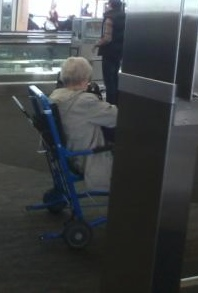
\includegraphics[width=7cm]{images/image034}
   \caption{From L to R: Wheelchair with small wheels, with big wheels and for aisle}
  \label{fig:34}
\end{figure}
\begin{figure}[h]
  \centering
     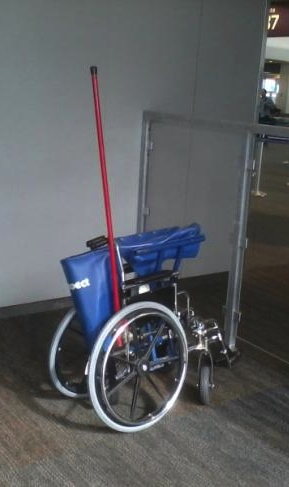
\includegraphics[width=7cm]{images/image035}
  \label{fig:35}
\end{figure}
\begin{figure}[h]
  \centering
     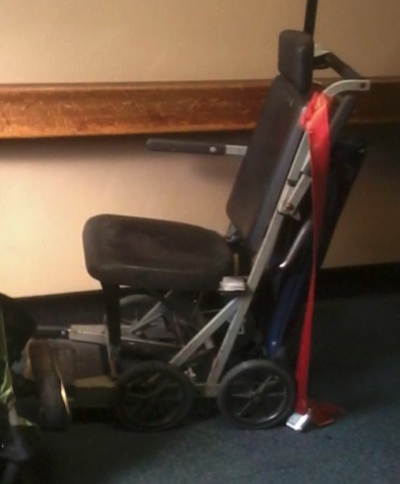
\includegraphics[width=7cm]{images/image036}
  \label{fig:36}
\end{figure}

  \item There are at least three types of wheelchairs like those in Figure 3 6 in an airport: those with small wheels which require someone else to push it, thus limiting the passenger’s independence, those with larger wheels that provide some level of independency since the passenger can conceivably wheel themselves around and aisle wheelchairs which are used for transporting passengers from a wheelchair in the jet way to their seats on the airplane.
  \item One is normally required to walk long distances to reach one’s gate. However, the airports we visited mitigated that problem by offering solutions like an electric cart that can carry up to 12 people (including the driver) and small buses for transportation outside the building, both shown in Figure 3 7.

\begin{figure}[h]
  \centering
     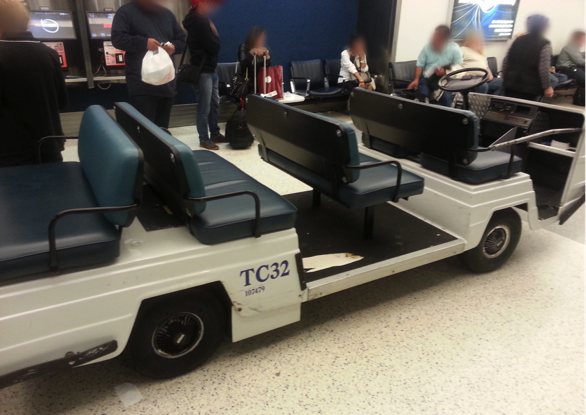
\includegraphics[width=7cm]{images/image037}
   \caption{From L to R: Cart for inside transportation and bus for outside transportation}
  \label{fig:37}
\end{figure}
\begin{figure}[h]
  \centering
     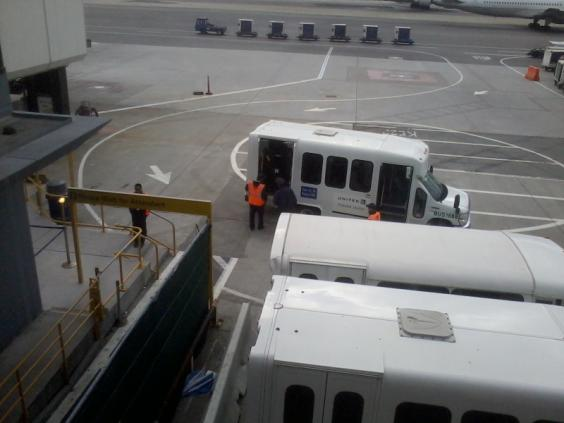
\includegraphics[width=7cm]{images/image038}
  \label{fig:38}
\end{figure}


  \item Finding the boarding gate can be a problem especially with last minute time changes, the increasing distance between gates and the difficulty of listening to the airport’s sound system.
  \item Removing all belongings when passing through security may be very difficult for some people. Although it is true that there is a special procedure for people with disabilities, the elderly did not have a special treatment.  The conveyor belt is too high, making it hard to place heavy belongings on the table. Plus, there is a lot of added social pressure to move extremely fast.
  \item It is very difficult to understand the airport’s sound system over the loud background noise, even if one has a good hearing.
  \item Some wheelchair users have to change wheelchairs more than once in airport during check-in and boarding.
  \item Finding one’s luggage and picking it up on baggage claim area is not as easy as one might imagine. The conveyor belt moves fast and the weight of the luggage is elevated, making it hard for someone with less than perfect mobility to easily achieve the task. Most of the time, there are no employees helping.

\begin{figure}[h]
  \centering
     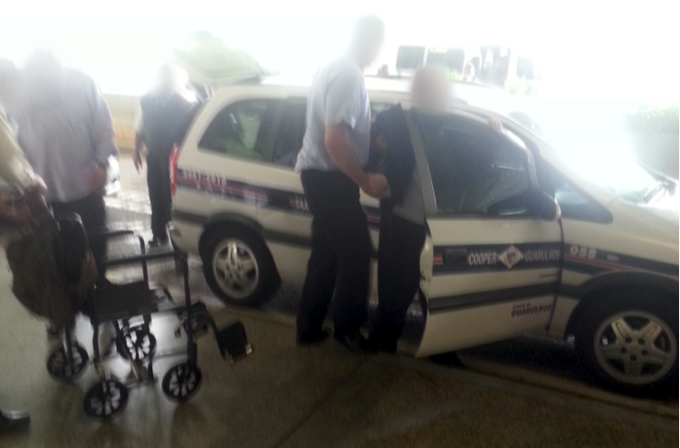
\includegraphics[width=7cm]{images/image039}
   \caption{Obese person being transferred from wheelchair to taxi.}
  \label{fig:39}
\end{figure}

  \item Although there a lot of taxis in airports, finding one that is accessible to people with reduced mobility is not as easy as one might expect. As a result, these people have to be assisted (and touched) by other people as seen in Figure 3 8.
\end{list}

\subsection{Airplane Observations}
\begin{enumerate}
  \item There should be an indicator to inform passengers if overhead luggage bin is full.
  \item Seat numbers should be marked more clearly because the numbers are too small.
  \item The food tray is very slippery causing contents to go rolling all over the place during flight. A better design would include a non-slippery surface.
  \item Attendant, light buttons and air control should be accessible and more intuitive to everyone. For a lot of people, it is very hard to reach all the way to the ceiling to press these buttons. In some aircraft, there is a button closer to the seat but unfortunately it is very difficult to see it. In other aircraft, the buttons are on the arm rest and get pressed accidentally all the time. 
  \item Seatbelts should be retractable to avoid tangling.
  \item Economy class seats need to be more ergonomic to provide more comfort for users, particularly for spine and lumbar support.
  \item Seats should have footrests to improve comfort for everyone and especially for shorter people. 
  \item The first row of seats should be more accessible to people with disabilities; the armrest should not be fixed since wheelchair users prefer to use these seats and aisle chair transfer is extremely difficult with an armrest in the way. 
  \item It is very difficult to understand pilot speaking in the airplane.
  \item The WC was not adapted for people with reduced mobility, it was small and cramped. 
  \item The height of the luggage bin makes it very difficult for everyone to store and retrieve a bag, especially for shorter people.
  \item  A suitable place to wait to go to the lavatory does not currently exist,  you are often blocking the aisle and hindering others from getting by you. 
  \item It is not possible to walk through the aisle when food is being served because of the dimensions of the cart/aisle.
  \item Attendants don’t provide enough time to eat. 
  \item Seats are not designed for children.
  \item There are no proper areas do dispose trash while seated (unless a flight attendant is walking by with a trash bag).
  \item In the lavatory it is not clear where each type of trash should be disposed where.
  \item The seat is too high for people with a short stature.
  \item The seat is too tight for obese people.
  \item The conventional seat belt is too tight for obese people. Flight attendants need to offer seat belt extensions but a lot of them aren’t even aware they exist.
\end{enumerate}

In order to represent the key observations in a more visual manner, the diagram represented in Figure 3 9 was created. A magnified version can be found in the Appendix – Diagram A2.

\begin{figure}[h]
  \centering
     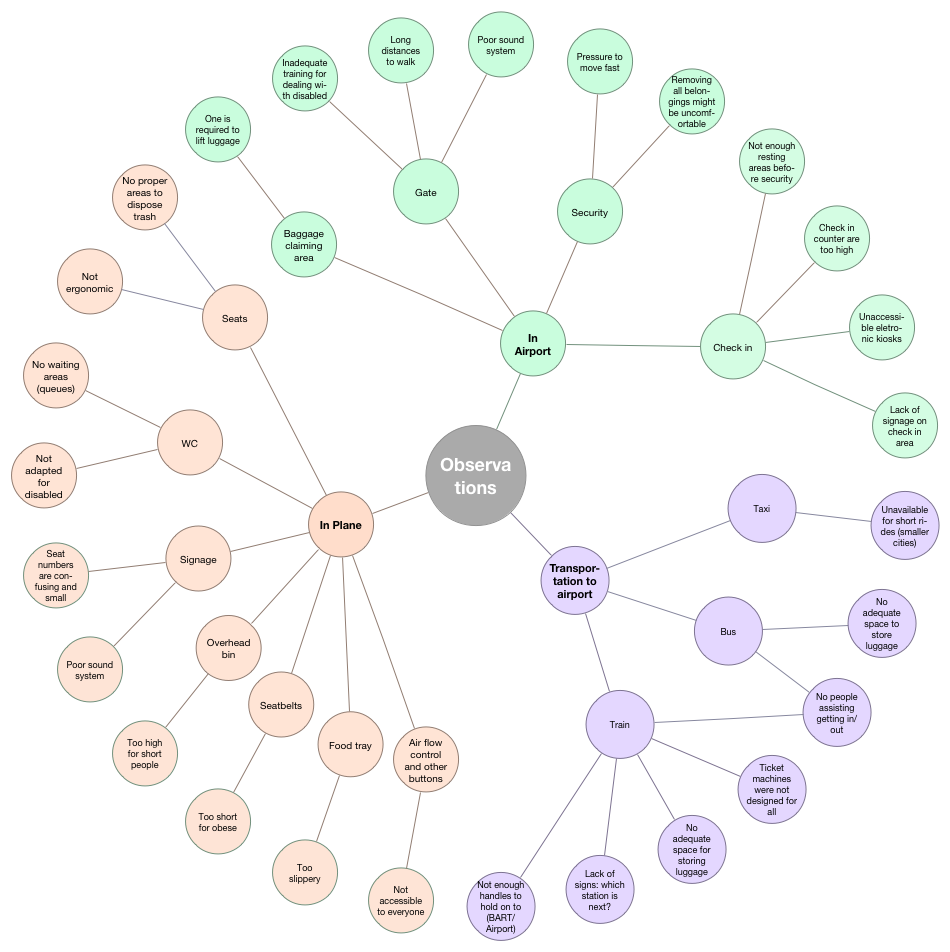
\includegraphics[width=7cm]{images/image040}
   \caption{Key observations diagram}
  \label{fig:40}
\end{figure}

\section*{Persona Development}
Our persona development was driven by our want to always keep the end user in mind. We recognize that this is a very human centered problem and want to ensure that we keep the human centered approach every step of the way. Through our interviews, observations and need-finding processes, we discovered our solution would actually have two critical users with very different problems and motivations. These users are Patty White, the grandma, and Juliette Fields, the flight attendant.

\subsection{Patty White, The Elderly Passenger}

\begin{figure}[h]
  \centering
     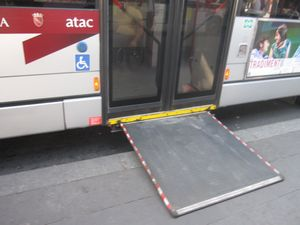
\includegraphics[width=7cm]{images/image041}
   \caption{Patty White, one of our design personas}
  \label{fig:41}
\end{figure}

We based Patty White, shown in Figure 3 5, on a compilation of characteristics from both our interviewees as well as characters in their stories. She is an older adult in her early 60s that has limited upper body strength and mobility. She is from Cleveland, Georgia and is a retired teacher. Her southern charm as well as her past experiences as an instructor make her a very well informed and easy going traveler, always eager to explain different rules and regulations because she is keen on helping the flight crew learn about people with disabilities. Patty is widowed and usually travels alone across the country to visit her grandchildren. For Patty, giving up on flying means giving up on family. She loves to cook and will often bring her family bags of baked and preserved goods as well as lots of toys for the kids, which means she usually travels with a lot of luggage.  Since Patty has just recently been dealing with her limited mobility, she is still learning to deal with being dependent on others. When flying, she is extremely uncomfortable because of the airplane seat’s lack of support and she needs to use the back of chairs to balance if she needs to move around the cabin.

\subsection{Juliette Fields, Flight Attendant}

The inspiration for our flight attendant arose from our many observations, past experiences and interviews. We know that the cabin crew plays an important part in the travel experience for disabled passengers and a great deal of horror stories comes from customer service issues. Thus, portraying this critical user and keeping their needs and motivations in mind is paramount as we design a solution. Juliette is in her late 20s, she doesn’t have a family and enjoys traveling around the world. She is fairly new to the airline industry and always follows protocol, she never goes above what is already listed. She does not have much experience with disabled passengers and is completely uneducated about their needs and abilities. 

\section{Benchmarking}
\section*{Analogous Solutions}
Part of the benchmarking phase of this project dealt with looking into other transportation and recreational areas where solutions have been implemented to accommodate those with limited mobility.  Cinemas, public buses, mobility buses, personal vehicles, tram and train platforms, and grocery stores were all areas that were examined as analogous situations to the problem we were presented with.

\subsection{Wheelchair and Passenger Transport}

\begin{figure}[h]
  \centering
     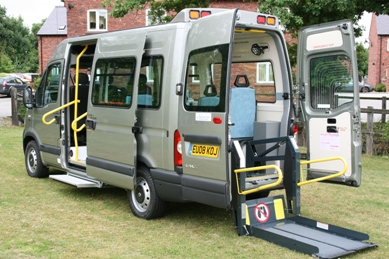
\includegraphics[width=7cm]{images/image042}
   \caption{Bus ramp used to assist entrance and exit onto bus. Source: http://www.romeinformation.it/en/guided-tours/rome-tours-for-disabled/}
  \label{fig:42}
\end{figure}

Public buses were researched first when looking at wheelchair and passenger transport given that public bus systems service more cities than other modes of public transportation.  Figure 3 6 shows a ramp that is either pulled out or automatically released from under the doors of the buses.  This creates a safer and more convenient entrance onto the bus for passengers in wheelchairs or passengers that have a difficult time making the large step onto the bus. 

\begin{figure}[h]
  \centering
     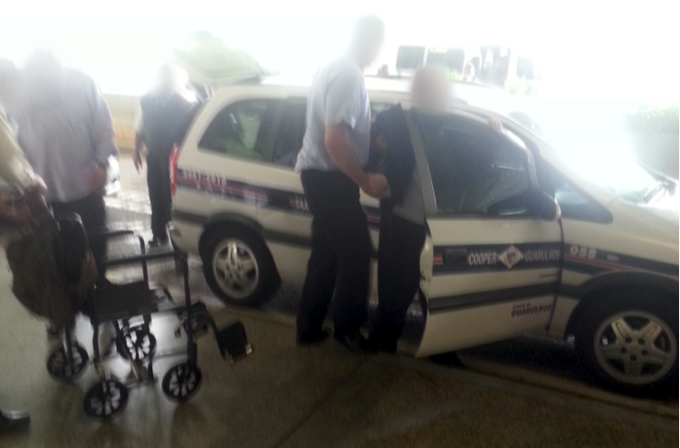
\includegraphics[width=7cm]{images/image039}
   \caption{Lift used to assist in loading process.}% Source: http://www.beckettcorp.co.uk/index_files/vehiclesforhireandsale.htm}
  \label{fig:39}
\end{figure}

Mobility buses or vans and personal vehicles were also examined as the accessibility features could be similar to the airplane issue being presented. These areas allow for more customization because they are designed to meet a specific need for a specific group of people.  Mobility vans and personal vehicles brought forth many plausible solutions that could be employed in addressing the problem.  Mobility vans/buses, just like public buses, utilized ramps or lifts to enter the vehicle Figure 3 12 show easy-access steps on a lift with extending handles for a mobility van.  

\begin{figure}[h]
  \centering
     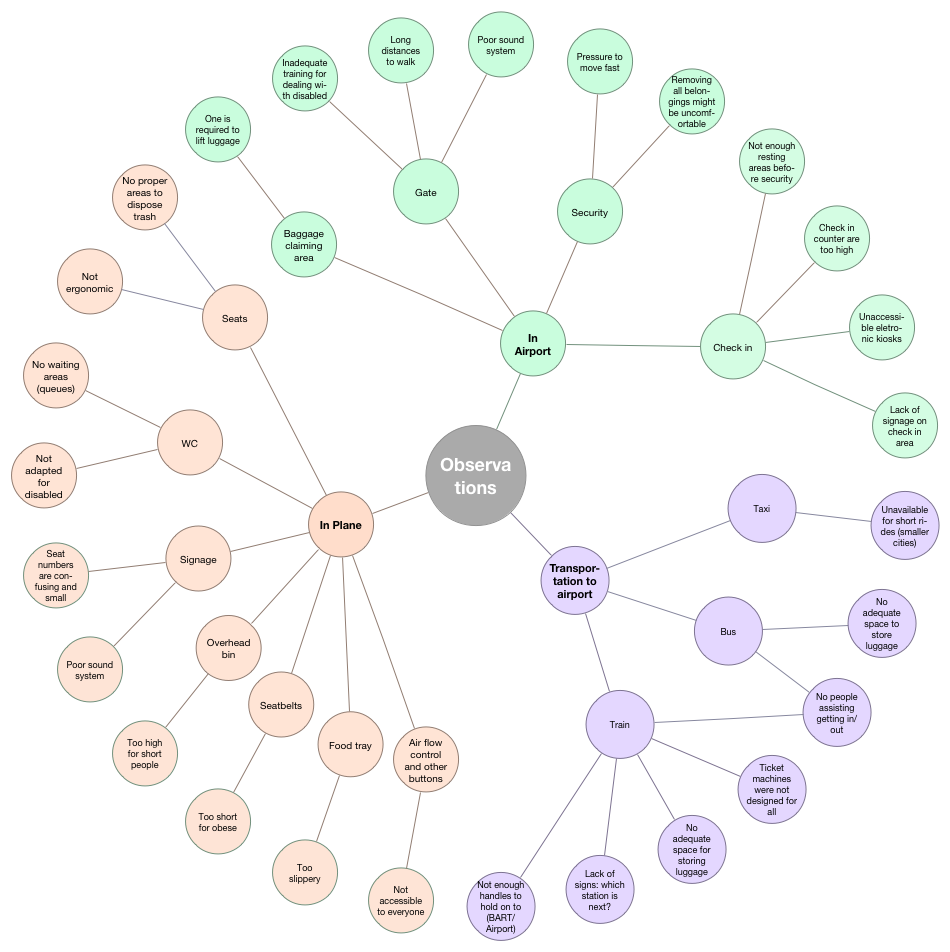
\includegraphics[width=7cm]{images/image040}
   \caption{Example of an aisle chair used to get wheelchair users into the plane.}
  \label{fig:40}
\end{figure}

Currently, a passenger that relies on a wheelchair will have to utilize an aisle chair like the one in Figure 3 13 when boarding and disembarking from a plane.  If the plane does not have a jet way, the passenger has to be carried up the stairs on the aisle chair by two people to get into the plane as shown in Figure 3 14. A passenger accustomed to being in their customized wheelchair will find the aisle chair and the carrying process very uncomfortable, unsecure, and embarrassing as evidenced by our research and interviews. We found that a variety of lifts were found that can be utilized to lift a wheelchair into a vehicle with just a push of a button once the wheelchair is latched down. Figure 3 15 shows a lift mechanism in a mobility van.  This lift mechanism raises the chair to the level of the van so that the wheelchair can then be wheeled onto the bus. This exact mechanism may not be suitable for aircrafts due to the increased height of the plane, but a mechanism that is similar and allowed for automated transfer from the platform to the aircraft could be utilized.  Figure 3 16 shows a lifting mechanism for a personal vehicle.  This mechanism brings the entire wheelchair into the can in a sideways position.  There is no manual transfer of the wheelchair from the platform to the car.  This kind of mechanism would allow for the wheelchair to be facing in the proper direction to go down the plane aisle without the need to maneuver the chair around to the correct position.

\begin{figure}[h]
  \centering
     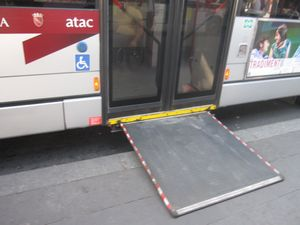
\includegraphics[width=7cm]{images/image041}
   \caption{Wheelchair user being carried up the stairs in an aisle chair.}% Source: http://www.disabilitytravel.com/airlines/air_carrier_act.htm}
  \label{fig:41}
\end{figure}

Lifting mechanisms are also utilized in tram and train stations as shown below in Figure 3 17.   A woman uses the lifting platform for her stroller to get to the tram platform. Women with strollers and young children can be analogous models for persons with disabilities because they require more assistance, have limited mobility, and require more room on the plane to move. 

\subsection{Wheelchair Latching}
Figure 3 13 shows a specific area on the bus that is reserved for passengers with disabilities.  The special area is a theme throughout most modes of public transportation beside aircraft.  The specialized seating area is equipped with the mounting or latching materials needed to secure a wheelchair to the floor so the person does not slide around when the bus turns or brakes. Passengers that are mobility-impaired or have a disability that does not require a wheelchair can sit in this area, which provides ease of getting on and off the bus. The seats in this area fold up and down so that passengers without disabilities can sit in this section when it is not needed for persons with disabilities.  This allows for this section of the bus to function for both groups of passengers without taking away seats.

These specialized seating areas allow for wheelchairs to be latched down. If power wheelchair or even manual wheelchair is being carried in a vehicle or on an airplane, a latching system needs to be used to secure the chair to the floor so that the chair can withstand normal movement and movement in the instance of a crash. The wheelchair in Figure 3 19 is secured on metal runners that run parallel to the wheels, similar to the runners on the aisle of the airplane.  Figure 3 20 shows the wheelchair being latched to metal runners that run perpendicular to the floor.  This could symbolize the latching area of a normal airplane seat that has been removed for the wheelchair. For both of these passengers, an addition has been added to the normal seatbelt to provide upper body protection in the case of forward acceleration due to braking or a crash. Seatbelt additions such as these are currently available on planes to passengers who need extra upper body support.

Safety is of the utmost importance when it comes to transporting a person, whether they are disabled or not. Therefore, the latching of the wheelchair must be done at the proper angles. Figure 3 21 shows the proper angles that need to be utilized when strapping down a wheelchair in a moving transportation medium.  These guidelines could be tested and modified to meet the airplane's G requirements and space, finding the optimal position that has the best level of safety for the passenger.

\subsection{Luggage Storage and Ease of Movement through Cabin}
For passengers with limited upper body strength, which is common among passengers with disabilities, getting luggage into the overhead compartments is a great challenge.  Many people who have difficulties feel that they disturb other passengers while trying to load their luggage or they are simply not able to get the luggage into the compartment. What if there was a way to make it easier to reach the overhead compartment? This is where grocery store accessibility features became an analogous situation.  Figure 3 17 shows a man utilizing a standing wheelchair that comes with a lift feature.  This feature allows for the person to maneuver through the store in a standing position and also reach goods from the top shelf.  By utilizing a stand-up wheelchair, the chair could easily fit down a plane aisle since the person is in a standing rather than sitting position.  Also, the chair allows the passenger to lift their bag into the overhead compartment with little to no effort without causing a disruption and remaining independent. We found that the need for independence is a common theme among disabled passenger. They do not want their disabilities to impede on their sense of independence. In addition, they do not want someone to think they cannot do something for themselves just because they have a disability. This idea of independence and individuality leads to the next topic of customization within analogous situations.  The stand-up wheelchair could also serve as a substitute for the aisle chair that is humiliating and uncomfortable to passengers. 

\subsection{Customization and Support}
Many people with disabilities have to customize their surroundings to fit their needs.  For persons that use a wheelchair regularly, this could mean using cushions or additional support to fit their body and their distribution of weight to prevent sores and arthritis. Figure 3 23 shows a wheelchair cushion that consists of both gel and air inserts to provide two support systems.  Cushions such as these are sometimes brought onto aircraft when a passenger has a long duration flight or knows they will be sitting the entire time.  Figure 3 24 shows an entire chair structure cushion that can be used to place on a chair or on a bench.  This cushion allows for back and lumbar support as well as weight distribution support, however this type of support system is seen less on a flight due to the misalignment between the seat back and the cushion back.  

Researching this area led to the finding of a chair, in Figure 3 25 that was specifically designed for children with disabilities to make the seats more comfortable, more accessible, and better fitting for the child during flights.  This chair provides upper body support by using neck supports to stabilize the head and neck and by using a seatbelt configuration that allows the body to stay upright without relying on the core muscles.  We found this attribute to be quite appealing since many persons of disabilities lose their core muscle strength due to lack of use and inability to exercise.  The chair has two back sections to provide needed lumbar support and hip support whereas the seat portion is thoroughly padded to provide better weight distribution.  The leg supports are configured so that the children's legs do not dangle the entire flight since this can lead to medical issues such as deep vein thrombosis.  The exact design of this chair would need to be modified for adult disabled passengers due to different needs and a bigger body frame.  However, the idea is still a feasible solution to the problem being presented.  Customizing an add-on airplane chair to fit the needs of the disabled passenger would allow for the disabled passenger to feel more comfortable but would not take away seats from any other passengers. 

The idea of customizing parts of a seat or a seat in general brought up a new solution area to look at including the eating trays, control boards, remotes, and pouches on the back of the chairs. Most of these items do not have an analogous situation that can be easily analyzed because they exist in personal cars and each make and model is different. However, we can use the current solutions implemented in power wheelchairs to explore options for food tray placement.  Figure 3 26 shows an add-on tray to a power wheelchair that allows for a person to have a tray closer to their body or in the green zone of the body.  This provides easier access and more support since the closer range activates the small muscle groups that control fine motor skills.  This solution that can be used on aircraft for persons who find the back of the seat or bring-up tray not stable enough for their body type and disability or for those that find they do not have a great amount of control.  This tray feature would add minimal weight to the aircraft and provide a sense of independence and control for the passenger.